\documentclass[
11pt, % The default document font size, options: 10pt, 11pt, 12pt
codirector, % Uncomment to add a codirector to the title page
]{charter} 


% El títulos de la memoria, se usa en la carátula y se puede usar el cualquier lugar del documento con el comando \ttitle
\titulo{Monitoreo y control de sistemas de bombeo de agua potable de pozos profundos} 

% Nombre del posgrado, se usa en la carátula y se puede usar el cualquier lugar del documento con el comando \degreename
\posgrado{Maestría en Sistemas Embebidos} 
%\posgrado{Carrera de Especialización en Internet de las Cosas} 
%\posgrado{Carrera de Especialización en Inteligencia Artificial}
%\posgrado{Maestría en Sistemas Embebidos} 
%\posgrado{Maestría en Internet de las cosas}
% IMPORTANTE: no omitir titulaciones ni tildación en los nombres, también se recomienda escribir los nombres completos (tal cual los tienen en su documento)
% Tu nombre, se puede usar el cualquier lugar del documento con el comando \authorname
\autor{Esp. Ing. Mario Fernando Aguilar Montoya}

% El nombre del director y co-director, se puede usar el cualquier lugar del documento con el comando \supname y \cosupname y \pertesupname y \pertecosupname
\director{Mg. Ing. Mauricio Barroso Benavides}
\pertenenciaDirector{FIUBA} 
%\codirector{Título y Nombre del codirector} % para que aparezca en la portada se debe descomentar la opción codirector en los parámetros de documentclass
%\pertenenciaCoDirector{FIUBA}

% Nombre del cliente, quien va a aprobar los resultados del proyecto, se puede usar con el comando \clientename y \empclientename
\cliente{Ing. Carlos Alvarado Cruz}
\empresaCliente{COSAALT RL}
 
\fechaINICIO{22 de junio de 2024}		%Fecha de inicio de la cursada de GdP \fechaInicioName
\fechaFINALPlan{17 de agosto de 2024} 	%Fecha de final de cursada de GdP
\fechaFINALTrabajo{8 de abril de 2025}	%Fecha de defensa pública del trabajo final


\begin{document}

\maketitle
\thispagestyle{empty}
\pagebreak


\thispagestyle{empty}
{\setlength{\parskip}{0pt}
\tableofcontents{}
}
\pagebreak


\section*{Registros de cambios}
\label{sec:registro}


\begin{table}[ht]
\label{tab:registro}
\centering
\begin{tabularx}{\linewidth}{@{}|c|X|c|@{}}
\hline
\rowcolor[HTML]{C0C0C0} 
Revisión & \multicolumn{1}{c|}{\cellcolor[HTML]{C0C0C0}Detalles de los cambios realizados} & Fecha      \\ \hline
0      & Creación del documento                                 &\fechaInicioName \\ \hline
1      & Se completa hasta el punto 9 inclusive                & {2} de {agosto} de 2024 \\ \hline
2      & Se completa el plan                & {12} de {agosto} de 2024 \\ \hline
3      & Se realizaron las correcciones del plan completo               & {16} de {agosto} de 2024 \\ \hline
%2      & Se completa hasta el punto 9 inclusive
%		  Se puede agregar algo más \newline
%		  En distintas líneas \newline
%		  Así                                                    & {día} de {mes} de 202X \\ \hline
%3      & Se completa hasta el punto 12 inclusive                & {día} de {mes} de 202X \\ \hline
%4      & Se completa el plan	                                 & {día} de {mes} de 202X \\ \hline

% Si hay más correcciones pasada la versión 4 también se deben especificar acá

\end{tabularx}
\end{table}

\pagebreak



\section*{Acta de constitución del proyecto}
\label{sec:acta}

\begin{flushright}
Buenos Aires, \fechaInicioName
\end{flushright}

\vspace{2cm}

Por medio de la presente se acuerda con el \authorname\hspace{1px} que su Trabajo Final de la \degreename\hspace{1px} se titulará ``\ttitle'' y consistirá en la implementación de un prototipo de un sistema para el monitoreo y control de un sistema de bombeo de agua potable. El trabajo tendrá un presupuesto preliminar estimado de 655 h de trabajo y un costo estimado de 47391.5 Bs, con fecha de inicio el \fechaInicioName\hspace{1px} y fecha de presentación pública el \fechaFinalName.

Se adjunta a esta acta la planificación inicial.

\vfill

% Esta parte se construye sola con la información que hayan cargado en el preámbulo del documento y no debe modificarla
\begin{table}[ht]
\centering
\begin{tabular}{ccc}
\begin{tabular}[c]{@{}c@{}}Dr. Ing. Ariel Lutenberg \\ Director posgrado FIUBA\end{tabular} & \hspace{2cm} & \begin{tabular}[c]{@{}c@{}}\clientename \\ \empclientename \end{tabular} \vspace{2.5cm} \\ 
\multicolumn{3}{c}{\begin{tabular}[c]{@{}c@{}} \supname \\ Director del Trabajo Final\end{tabular}} \vspace{2.5cm} \\
\end{tabular}
\end{table}




\section{1. Descripción técnica-conceptual del proyecto a realizar}
\label{sec:descripcion}

En los últimos años la tendencia tecnológica se ha orientado hacia la creación de dispositivos electrónicos conectados a internet, lo que permite la implementación de una amplia variedad de nuevas aplicaciones.

Cossalt RL es una cooperativa que brinda el servicio de agua potable en la ciudad de Tarija. Actualmente la cooperativa posee 50 sistemas de bombeo de agua de pozos distribuidos por toda la ciudad para suministrar agua potable a los usuarios de cada zona. La mayoría de los sistemas son manuales, esto quiere decir que se necesita un operario encargado de encender y apagar las bombas de agua en funcion del nivel de agua en los tanques de almacenamiento.

El objetivo principal del proyecto es el desarrollo de un sistema capaz de realizar lecturas de consumo eléctrico de las bombas, presión del agua en las tuberías, nivel del tanque de almacenamiento y transmision de los datos obtenidos a una plataforma IoT mediante el uso de un módulo de comunicación GSM/GPRS. El sistema también controlará el encendido y apagado de las bombas de forma automática a partir de las lecturas de los sensores. La plataforma IoT permitirá almacenar los datos, crear paneles de visualización y controlar actuadores(bombas de agua). También se mostrarán los datos obtenidos en un display ubicado en el panel de control.
En la figura \ref{fig:diagra_sistema} se puede observar el diagrama de bloques del sistema.

El proyecto permitirá al cliente disminuir el desperdicio de agua que ocurre durante el proceso de bombear agua desde los pozos profundos a los tanques de almacenamiento, también ayudará a detectar de forma temprana posibles rupturas en las tuberías. Al tener un monitoreo y control automático del encendido y apagado de las bombas se prevé un disminución del consumo eléctrico.

\begin{figure}[hpb]
	\centering 
	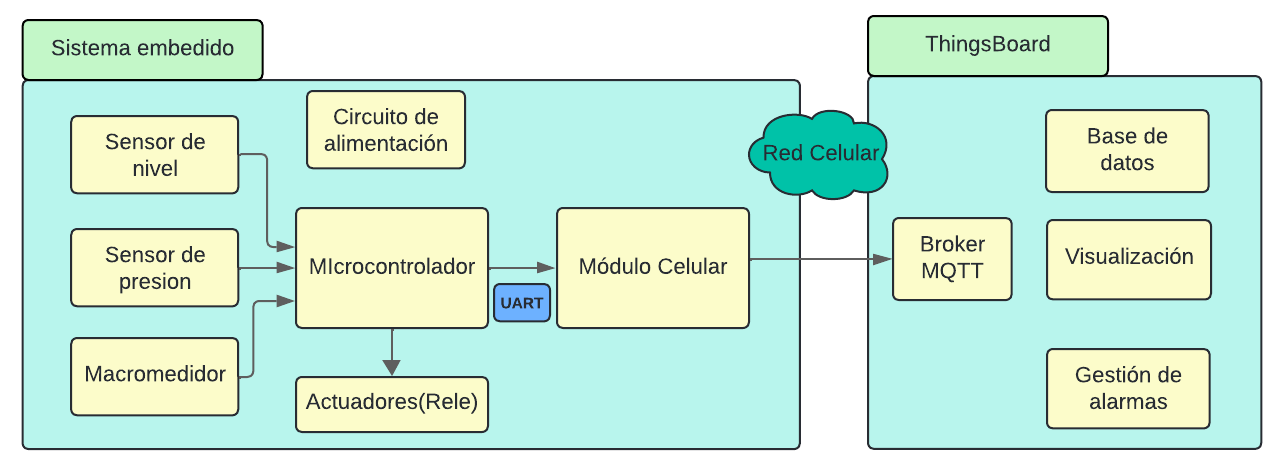
\includegraphics[width=15cm, height=8.5cm]{./Figuras/d_sistema.png}
	\caption{Diagrama en bloques del sistema.}
	\label{fig:diagra_sistema}
\end{figure}
\vspace{2cm}



\section{2. Identificación y análisis de los interesados}
\label{sec:interesados}

\begin{table}[ht]
%\caption{Identificación de los interesados}
%\label{tab:interesados}
\begin{tabularx}{\linewidth}{@{}|l|X|X|l|@{}}
\hline
\rowcolor[HTML]{C0C0C0} 
Rol           & Nombre y Apellido & Organización 	& Puesto 	\\ \hline
Cliente       & \clientename      &\empclientename	& Operador de sistema de bombeo      	\\ \hline
Responsable   & \authorname       & FIUBA        	& Alumno 	\\ \hline
Orientador    & \supname	      & - 				& Director del Trabajo Final \\ \hline
Usuario final & Operarios         & COSAALT RL            	& -      	\\ \hline
\end{tabularx}
\end{table}

\begin{itemize}
	\item Orientador: el Mg. Ing. Mauricio Barroso Benavides tiene mucha experiencia en el desarrollo de proyectos IoT, será una guía para el desarrollo del firmware y del hardware del embebido. Es exigente con los tiempos y la
	calidad del desarrollo del proyecto.
\end{itemize}



\section{3. Propósito del proyecto}
\label{sec:proposito}
El propósito del proyecto es desarrollar un sistema que sea capaz de monitorear y controlar parámetros relevantes en un sistema de bombeo de agua, con la finalidad de disminuir el consumo energético de las bombas  y el desperdicio de agua potable.

\section{4. Alcance del proyecto}
\label{sec:alcance}
El proyecto incluye:
\begin{itemize}
	\item Diseño e implementación del PCB, esto incluye todas las etapas desde el diseño de los esquemáticos hasta el envío para la fabricación y ensamblaje, finalmente las pruebas preliminares de funcionamiento.
	\item Desarrollo del firmware del microcontrolador basado en un sistema operativo de tiempo real.
	\item Configuración de la plataforma IoT para la visualización, almacenamiento, gestión de alarmas.
\end{itemize}
El proyecto no incluye:
\begin{itemize}
	\item Diseño y fabricación del gabinete que aloja al dispositivo.
	\item Manuales de instalación y de usuario del dispositivo.
\end{itemize}

\newpage
\section{5. Supuestos del proyecto}
\label{sec:supuestos}

\begin{itemize}
	\item El tiempo de fabricación y ensamblaje de los PCBs de prueba estará dentro de lo planeado.
	\item El tiempo de importación de los módulos y componentes estarán dentro del tiempo esperado.
	\item El presupuesto no superará en gran medida lo estimado.
	\item El tiempo disponible para trabajar en el proyecto será el adecuado para cumplir con
	los objetivos.
 
\end{itemize}

\section{6. Requerimientos}
\label{sec:requerimientos}
\begin{enumerate}
	\item Requerimientos funcionales:
		\begin{enumerate}
			\item Requerimientos de firmware
			\begin{enumerate} 
				\item El firmware debe estar sobre un RTOS.
				\item Se deberá llevar control de los cambios bajo el sistema de control de versiones Git.
				\item El firmware debe poder suscribirse y publicar en tópicos de un broker MQTT.
				\item El firmware debe comunicarse con el módulo GSM/GPRS mediante algun protocolo serial.
				\item El firmware debe poder obtener las lecturas de los sensores.
				\item El firmware debe poder actualizarse de forma remota.
				\item Se deben desarrollar los drivers para los sensores.
				\item Se debe hacer test unitarios para los drivers.
			\end{enumerate}
			\item Requerimientos de hardware
			\begin{enumerate} 
				\item El PCB debe tener un circuito de acondicionamiento para una entrada RS485.
				\item El PCB debe tener un circuito de acondicionamiento para una entrada de 4-20 mA.
				\item El PCB debe tener un circuito de acondicionamiento para una entrada de 0-10 V.
				\item Debe contar con una display.
			\end{enumerate}			
			\item Requerimientos de la plataforma IoT
			\begin{enumerate} 
				\item Debe mostrar los valores de los sensores.
				\item Debe mostrar el estado de los actuadores.
				\item Debe contar con botones para controlar los actuadores.
				\item Debe almacenar los datos.
				\item Debe poder establecer reglas y alarmas. 
			\end{enumerate}
			\item Requerimientos de documentación
			\begin{enumerate} 
				\item Se debe presentar un informe de avance del proyecto.
				\item Se debe presentar una memoria técnica al final del proyecto.
			\end{enumerate}
		\end{enumerate}

\end{enumerate}

\newpage
\section{7. Historias de usuarios (\textit{Product backlog})}
\label{sec:backlog}

El criterio para asignar los puntos a las historias de usuario es el siguiente:
\begin{itemize}
	\item Cantidad de trabajo a realizar 
	\begin{itemize}
		\item Bajo: peso 1
		\item Medio: peso 3
		\item Alto: peso 5 
	\end{itemize}
	\item Complejidad del trabajo a realizar
	\begin{itemize}
		\item Bajo: peso 1
		\item Medio: peso 3
		\item Alto: peso 5  
	\end{itemize}
	\item Riesgo o incertidumbre del trabajo a realizar
	\begin{itemize}
		\item Bajo: peso 1
		\item Medio: peso 3
		\item Alto: peso 5  
	\end{itemize}
\end{itemize}

Historia de usuario 1:``Como operador quiero ver en una pantalla local las lecturas de los sensores para accionar algún actuador en base a estas lecturas''
\begin{itemize}
	\item Dificultad: medio(3) 
	\item Complejidad: medio(3)
	\item Riesgo: bajo(1)  
\end{itemize}
Story point=(3+3+1)=7

Historia de usuario 2:``Como operador quiero recibir alertas cuando las lecturas de los sensores sobrepasen valores permitidos''
\begin{itemize}
	\item Dificultad: medio(3) 
	\item Complejidad: medio(3)
	\item Riesgo: alto(5)
\end{itemize}
Story point=(3+3+5)=11

Historia de usuario 3:``Como operador quiero poder visualizar la información que genera el sistema en un dashboard
que pueda ser accedido mediante internet''
\begin{itemize}
	\item Dificultad: medio(3) 
	\item Complejidad: medio(3)
	\item Riesgo: bajo(1)  
\end{itemize}
Story point=(3+3+1)=7

\section{8. Entregables principales del proyecto}
\label{sec:entregables}

\begin{itemize}
	\item Documentación en formato pdf de los esquemáticos y planos del PCB.
	\item Código fuente del firmware.
	\item Prototipo.
	\item Documentación del proyecto.
\end{itemize}

\section{9. Desglose del trabajo en tareas}
\label{sec:wbs}

\begin{enumerate}
\item Documentación del proyecto (60 h)
	\begin{enumerate}
	\item Escribir la planificación del proyecto (40 h)
	\item Especificación de requisitos del firmware (10 h)
	\item Definición de las pruebas de aceptación (10 h)
	\end{enumerate}
\item Búsqueda de material bibliográfico  (45 h)
	\begin{enumerate}
	\item Buscar hojas de datos de todos los componentes (15 h)
	\item Estudiar el funcionamiento de cada uno de los componentes (15 h)
	\item Investigar sobre dispositivos con funciones similares (15 h)
	\end{enumerate}
\item Diseño del hardware del sistema (155 h)
	\begin{enumerate}
	\item Selección de componentes (15 h)
	\item Diseño del esquemático (60 h)
	\begin{enumerate}
		\item Diseño del esquemático para el microcontrolador (40 h)
		\item Diseño del esquemático de los circuito de acondicionamiento para las entradas (10 h)
		\item Diseño del esquemático de los circuito de acondicionamiento para las salidas (10 h)
	\end{enumerate}
	\item Diseño de los símbolos (20 h)
	\item Diseño del PCB (60 h)
	\begin{enumerate}
		\item Ubicación de los componentes en el PCB (20 h)
		\item Ruteo del PCB (40 h)
	\end{enumerate}
	\end{enumerate}
\item Desarrollo del firmware (175 h)
	\begin{enumerate}
	\item Diseño de la arquitectura del firmware (25 h)
	\item Desarrollo de los drivers del firmware (70 h)
	\begin{enumerate}
		\item Desarrollo del driver para el sensor de presión (20 h)
		\item Desarrollo del driver para el sensor de nivel (20 h)
		\item Desarrollo del driver para el macromedidor (10 h)
		\item Desarrollo del driver para el medidor de energía (20 h)
	\end{enumerate}
	\item Desarrollar el módulo de la aplicación (80 h)
	\begin{enumerate}
		\item Creación de las tareas en el RTOS (40 h)
		\item Creación de los recursos del RTOS (40 h)
	\end{enumerate}
	\end{enumerate}
\item Configuración de la plataforma IoT (70 h)
    \begin{enumerate}
		\item Diseño de la interfaz gráfica en la plataforma IoT (40 h)
		\item Configuración de la base de datos, alarmas y reglas (30 h)
	\end{enumerate}
\item Testing (30 h)	
    \begin{enumerate}
		\item Testeo eléctrico del PCB (10 h)
		\item Testeo del firmware (10 h)
		\item Depuración del firmware (10 h)
	\end{enumerate}
\item Cierre del proyecto (120 h)	
    \begin{enumerate}
		\item Informes de avance del proyecto (20 h)
		\item Elaboración de la memoria técnica del trabajo final (80 h)
		\begin{enumerate}
			\item Elaboración de la memoria hasta el capítulo 2 (40 h)
			\item Elaboración de la memoria del capítulo 3 al 6 (40 h)
		\end{enumerate}
		\item Presentación final del proyecto (20 h)
	\end{enumerate}


\end{enumerate}

Cantidad total de horas: (655 h)

\newpage
\begin{landscape}
\section{10. Diagrama de Activity On Node}
\label{sec:AoN}
Se resalta con color rojo las flechas que corresponden al camino crítico y a las que hay que prestar mayor atención para evitar retrasos. La suma del camino crítico estima un tiempo de desarrollo del proyecto de 450 h.

\begin{figure}[htpb]
	\centering 
	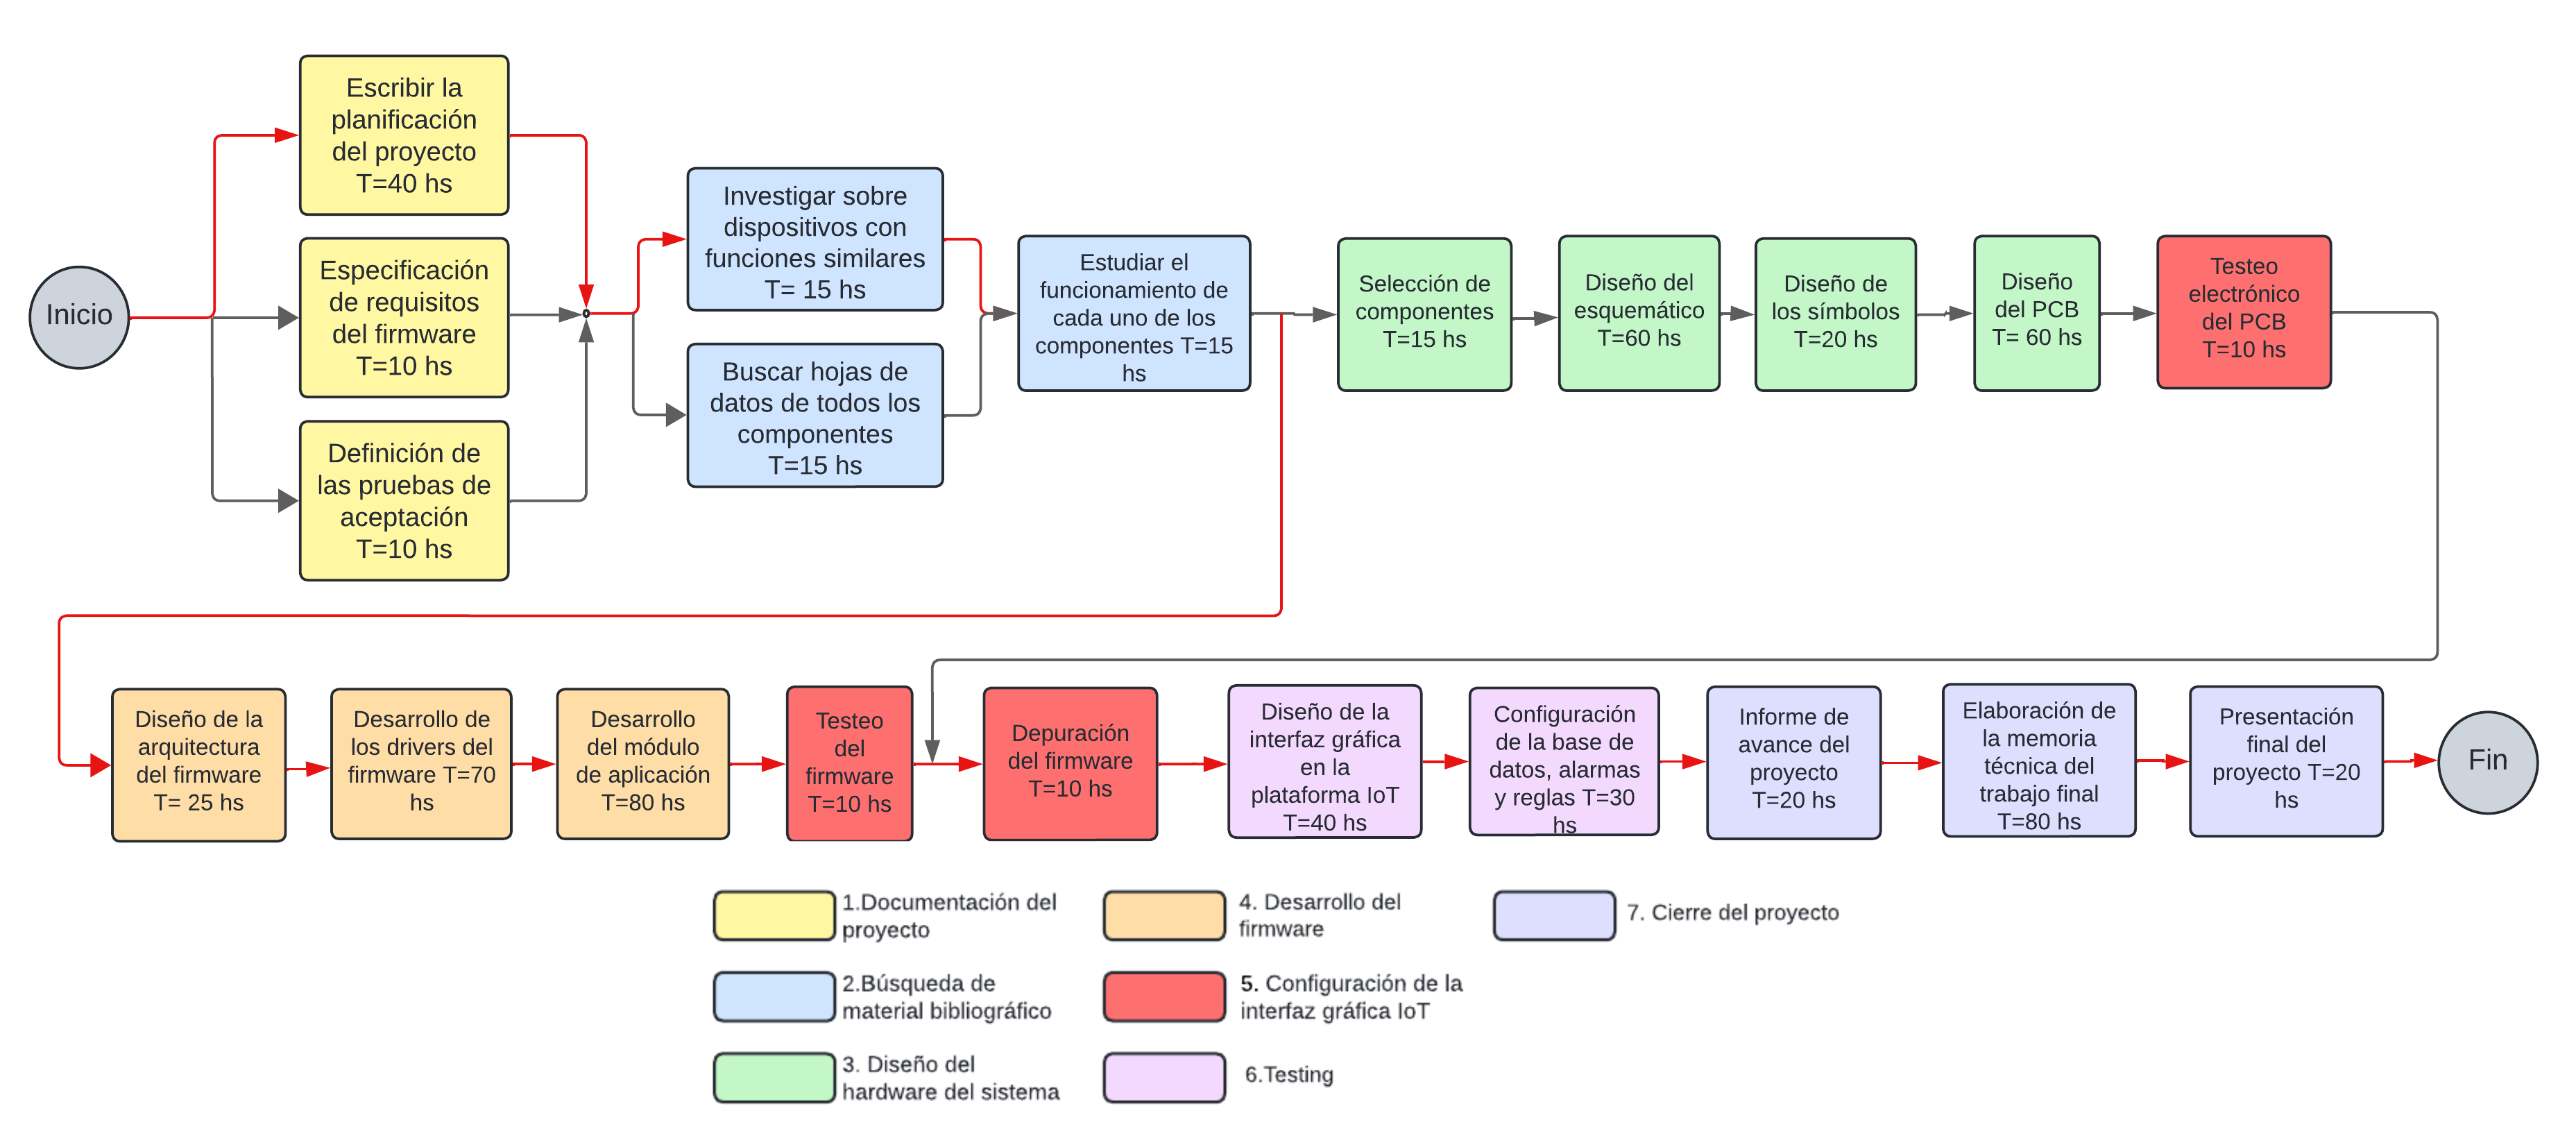
\includegraphics[width=22cm, height=11cm]{./Figuras/diagramaAc.png}
	\caption{Diagrama de \textit{Activity on Node}.}
	\label{fig:AoN}
\end{figure}
\end{landscape}

\newpage
\begin{landscape}
\section{11. Diagrama de Gantt}
\label{sec:gantt}
\begin{figure}[htpb]
	\centering 
	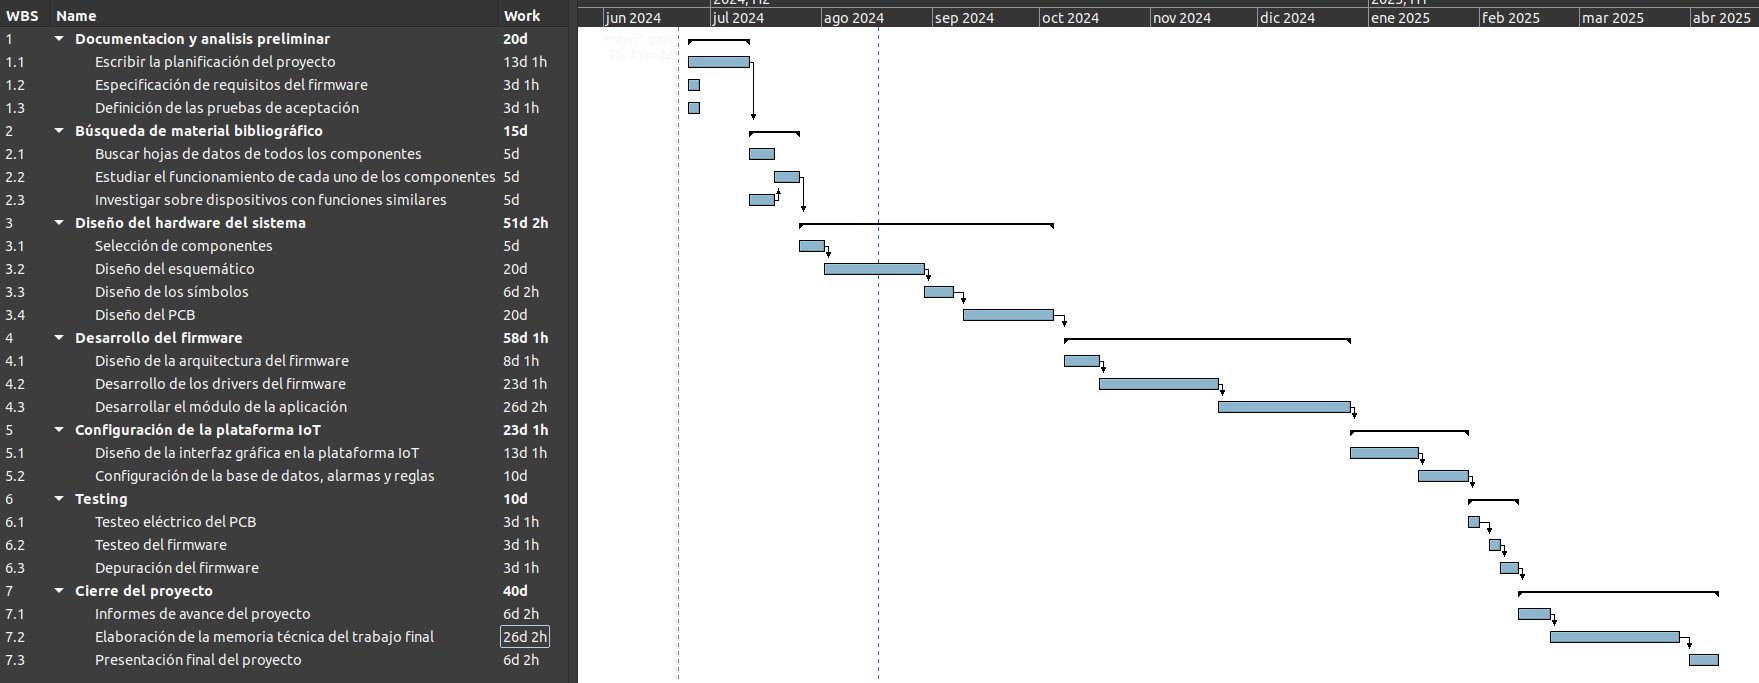
\includegraphics[width=24cm, height=11cm]{./Figuras/ganntfinal2.png}
	\caption{Diagrama de \textit{Activity on Node}.}
	\label{fig:d_gantt}
\end{figure}
\end{landscape}

\section{12. Presupuesto detallado del proyecto}
\label{sec:presupuesto}
Los precios expresados en la siguiente tabla se encuentran en Bolivianos Bs.

\begin{table}[htpb]
\centering
\begin{tabularx}{\linewidth}{@{}|X|c|r|r|@{}}
\hline
\rowcolor[HTML]{C0C0C0} 
\multicolumn{4}{|c|}{\cellcolor[HTML]{C0C0C0}COSTOS DIRECTOS} \\ \hline
\rowcolor[HTML]{C0C0C0} 
Descripción &
  \multicolumn{1}{c|}{\cellcolor[HTML]{C0C0C0}Cantidad} &
  \multicolumn{1}{c|}{\cellcolor[HTML]{C0C0C0}Valor unitario} &
  \multicolumn{1}{c|}{\cellcolor[HTML]{C0C0C0}Valor total} \\ \hline
 Tarjeta de desarrollo&
  \multicolumn{1}{c|}{1}&
  \multicolumn{1}{c|}{150} &
  \multicolumn{1}{c|}{150} \\ \hline
Módulo de comunicación GSM/GPRS&
  \multicolumn{1}{c|}{1} &
  \multicolumn{1}{c|}{350} &
  \multicolumn{1}{c|}{350} \\ \hline
Componentes electrónicos para el PCB&
  \multicolumn{1}{c|}{1} &
  \multicolumn{1}{c|}{400} &
  \multicolumn{1}{c|}{400} \\ \hline 
Fabricación y emsamblaje del PCB&
  \multicolumn{1}{c|}{5} &
  \multicolumn{1}{c|}{209} &
  \multicolumn{1}{c|}{1045} \\ \hline 
Pantalla nextion&
  \multicolumn{1}{c|}{1} &
  \multicolumn{1}{c|}{260} &
  \multicolumn{1}{c|}{260} \\ \hline 
Caja de la tarjeta PCB&
  \multicolumn{1}{c|}{1} &
  \multicolumn{1}{c|}{250} &
  \multicolumn{1}{c|}{250} \\ \hline
Horas de ingeniería &
  \multicolumn{1}{c|}{680} &
  \multicolumn{1}{c|}{50} &
  \multicolumn{1}{c|}{34000} \\ \hline  

\multicolumn{3}{|c|}{SUBTOTAL}   &
  \multicolumn{1}{c|}{36455} \\ \hline
\rowcolor[HTML]{C0C0C0} 
\multicolumn{4}{|c|}{\cellcolor[HTML]{C0C0C0}COSTOS INDIRECTOS} \\ \hline
\rowcolor[HTML]{C0C0C0} 
Descripción &
  \multicolumn{1}{c|}{\cellcolor[HTML]{C0C0C0}Cantidad} &
  \multicolumn{1}{c|}{\cellcolor[HTML]{C0C0C0}Valor unitario} &
  \multicolumn{1}{c|}{\cellcolor[HTML]{C0C0C0}Valor total} \\ \hline
\multicolumn{1}{|l|}{30 \% de los costos directos} &
   1&
   1&10936.5
   \\ \hline
\multicolumn{3}{|c|}{SUBTOTAL} &
  \multicolumn{1}{|c|}{10936.5} \\ \hline
\rowcolor[HTML]{C0C0C0}
\multicolumn{3}{|c|}{TOTAL} &47391.5
   \\ \hline
\end{tabularx}%
\end{table}


\section{13. Gestión de riesgos}
\label{sec:riesgos}
a) Identificación de los riesgos y estimación de sus consecuencias:

Riesgo 1: detección de errores en el esquemático o el ruteo del PCB ya habiendo fabricado los prototipos.
\begin{itemize}
	\item Severidad (9): se retrasa el proyecto por unas semanas hasta volver a mandar a fabricar los PCBs nuevamente, tambien el presupuesto estimado para los PCBs se duplicara.
	\item Probabilidad de ocurrencia (4): dada la moderada experiencia del alumno es posible que ocurra.
\end{itemize}  

Riesgo 2: mala estimación de la planificación.
\begin{itemize}
	\item Severidad (6): el proyecto sufrirá varios cambios y retrasos en la ejecución.
	\item Probabilidad de ocurrencia (6): el encargado del proyecto no cuenta con experiencia en planificación de proyectos IoT.
\end{itemize}

Riesgo 3: retraso en la programación del firmware.
\begin{itemize}
	\item Severidad (7): retrasos en el proyecto debido a que el firmware es una parte fundamental en el momento de la integración e implementación del prototipo.
	\item Probabilidad de ocurrencia (5): el encargado del proyecto le falta experiencia con la arquitectura del microcontrolador y el uso de RTOS.
\end{itemize}  

Riesgo 4: retraso en la fabricación y ensamblaje de los PCBs.
\begin{itemize}
	\item Severidad (5): antes de mandar el PCBs se prueba el firmware en un prototipo.
	\item Probabilidad de ocurrencia (4): los PCBs se mandarán a fabricar y ensamblar a una empresa china. 
\end{itemize}

Riesgo 5: pérdida o daño de los archivos asociados al proyecto.
\begin{itemize}
	\item Severidad (7): al perder los archivos del proyecto se tendrá que volver reiniciar diseños.
	\item Probabilidad de ocurrencia (1): se llevará un control de versiones con los documentos del proyecto.
\end{itemize}  

b) Tabla de gestión de riesgos: 

\begin{table}[htpb]
\centering
\begin{tabularx}{\linewidth}{@{}|X|c|c|c|c|c|c|@{}}
\hline
\rowcolor[HTML]{C0C0C0} 
Riesgo & S & O & RPN & S* & O* & RPN* \\ \hline
Detección de errores en el esquemático o el ruteo del PCB ya habiendo fabricado los prototipos&  9&   4&     36&    9&    3&      27\\ \hline
Mala estimación de la planificación      &   6&   6&     36&    6&    4&      24\\ \hline
Retraso en la programación del firmware       &   7&   5&     35&    &    &      \\ \hline
Retraso en la fabricación y ensamblaje de los PCBs       &   5&   4&     20&    &    &      \\ \hline
Pérdida o daño de los archivos asociados al proyecto      &   7&   1&     7&    &    &      \\ \hline
\end{tabularx}%
\end{table}

Criterio adoptado: 

Se tomarán medidas de mitigación en los riesgos cuyos números de RPN sean mayores o iguales a 36.

Nota: los valores marcados con (*) en la tabla corresponden luego de haber aplicado la mitigación.

c) Plan de mitigación de los riesgos que originalmente excedían el RPN máximo establecido:
 
Riesgo 1*: se revisará minuciosamente los esquemáticos, el ruteo del PCB, y se buscará ayuda en algún ingeniero que tenga experiencia en desarrollo de circuitos impresos en proyectos de estas características.
  \begin{itemize}
	\item Severidad (9): no cambia.
	\item Probabilidad de ocurrencia (3): será menor al contar con ayuda de profesionales expertos en el tema.
\end{itemize}

Riesgo 2*: se consultará con el director en el momento de realizar la planificación para ajustar los tiempos de las tareas de acuerdo a su experiencia en este tipo de proyectos.
  \begin{itemize}
	\item Severidad (6): no cambia.
	\item Probabilidad de ocurrencia (4): se reduce el riesgo de hacer una mala planificación.
\end{itemize}


\section{14. Gestión de la calidad}
\label{sec:calidad}
Para cada uno de los requerimiento funcionales, se lista su respectiva validación y verificación. Las mismas llevadas a cabo por el responsable del proyecto.

\begin{itemize} 
	\item Req \#1: el firmware debe estar sobre un RTOS.
	\begin{itemize}
		\item Verificación: envio de datos por colas entre tareas.
		\item Validación: mostrar el intercambio de datos entre tareas por monitor serial. 
	\end{itemize}

	\item Req \#2: se deberá llevar control de los cambios bajo el sistema de control de versiones Git.
	\begin{itemize}
		\item Verificación: utilizar una consola de comandos para mandar comandos Git en los archivos del proyecto.
		\item Validación: mostrar los realeses realizados durante el proyecto.  
	\end{itemize}

	\item Req \#3: el firmware debe poder suscribirse y publicar en tópicos de un broker MQTT.
	\begin{itemize}
		\item Verificación: publicar datos a un tópico del broker MQTT.
		\item Validación: visualizar los datos en la interfaz gráfica en la plataforma IoT. 
	\end{itemize}

	\item Req \#4: el firmware debe comunicarse con el módulo GSM/GPRS mediante algun protocolo serial.
	\begin{itemize}
		\item Verificación: mandar comandos AT por puerto serial y esperar la respuesta del módulo.
		\item Validación: visualizar las respuesta del módulo en un monitor serial.  
	\end{itemize}

	\item Req \#5: se deben realizar los drivers para los sensores.
	\begin{itemize}
		\item Verificación: hacer un test unitario para cada driver.
		\item Validación: mostrar los resultados de cobertura en GCOV. 
	\end{itemize}

	\item Req \#6: el PCB debe tener un circuito de acondicionamiento para una entrada RS485.
	\begin{itemize}
		\item Verificación: hacer la lectura del sensor conectado por RS485.
		\item Validación: inspección por parte de cliente del circuito en el PCB.  
	\end{itemize}

	\item Req \#7: debe contar con una display.
	\begin{itemize}
		\item Verificación: mandar datos al display para visualizarlos.
		\item Validación: mostrar lecturas de los sensores en gráficas en el display.  
	\end{itemize}

	\item Req \#8: debe mostrar los valores de los sensores.
	\begin{itemize}
		\item Verificación: mandar datos leídos de los sensores a un tópico por MQTT a la plataforma.
		\item Validación: entrar a la plataforma IoT y visualizar los datos. 
	\end{itemize}

	\item Req \#9: debe contar con botones para controlar la actuadores.
	\begin{itemize}
		\item Verificación: visualizar los datos recibidos en un monitor serial al momento de presionar un botón en la plataforma IoT.
		\item Validación: oprimir un botón en la interfaz y visualizar la activación de un actuador. 

	\item Req \#10: requerimientos de documentación.
	\begin{itemize}
		\item Verificación: verificar que se haya presentado el informe de avance y la memoria técnica del proyecto.
		\item Validación: revisar que se cumplieran los requerimientos estipulados en el plan de proyectos. 
	\end{itemize}
\end{itemize}
\end{itemize}

\section{15. Procesos de cierre}    
\label{sec:cierre}

\begin{itemize}
	\item Pautas de trabajo que se seguirán para analizar si se respetó el Plan de Proyecto original:
	\begin{itemize}
		\item Encargado: Ing. Mario Aguilar Montoya
		\item Procedimiento: durante el proceso de cierre se evaluará si se ha cumplido los plazos
		de entrega y ejecución de cada tarea planteada en el Plan de Proyecto. En el caso de hallar requerimientos incumplidos y/o retrasos en las
		tareas se evaluarán las causa y se propondrán acciones para evitarlo en futuros
		proyectos.
	\end{itemize}
	\item Identificación de las técnicas y procedimientos útiles e inútiles que se emplearon, los problemas que surgieron y cómo se solucionaron:
	\begin{itemize}
		\item Encargado: Ing. Mario Aguilar Montoya
		\item Procedimiento: se evaluarán los procedimientos utilizados en función a su utilidad
		y eficiencia para alcanzar los objetivos predefinidos.
	\end{itemize}
	\item Acto de cierre:
	\begin{itemize}
		\item Encargado: Ing. Mario Aguilar Montoya
		\item Procedimiento: se realizará la defensa pública del trabajo final ante el jurado, posterior a esto se
		procederá a agradecer a todos los que ayudaron a realizar el proyecto, director del
		trabajo, miembros del jurado y autoridades de la CESE.
	\end{itemize}
\end{itemize}

\end{document}


\end{document}